\subsection{Similarity with Probabilistic Automatons}
\label{sec:hmm_vs_pa}
The Pautomac competition data has been generated by \gls{pa}s. Since we are concerned with the problem of learning the parameters of a \gls{hmm} that best describes the training data we are given, we need to reason about the difference between \gls{hmm}s and probabilistic automatons. The \gls{pa} is more or less equivalent to the \gls{hmm} in the way it works. Each state in a \gls{hmm} has a probability of emitting a given symbol, while the \gls{pa} defines these emission probabilities as a label on the transitions between states~\cite{pautomacTR}. This difference does however still allow for converting back and forth between the two models.
A more significant difference is the \gls{pa}'s use of halting probabilities, which for each state defines the probability of halting immediately after transitioning to that state. Because of the halting probabilities, the \gls{pa} generates of strings of finite length, as long as we assume that all states can reach a state that has a halting probability greater than 0. In contrast to the \gls{pa}, the \gls{hmm} does not have halting probabilities. Thus, the \gls{hmm} generates infinite sequences. However, the \gls{hmm} can easily be modified to include halting probabilities, just as the \gls{pa} can be modified to discard the halting probabilities. In both ways, we get two equivalent models.

In \ref{fig:model-with-and-without-stop-symbols}, the model to the left is a \gls{pa}, and the model to the right is a \gls{hmm}.
Notice that for the \gls{pa}, the probability of stopping when entering the state A is written inside the circle.

\begin{figure}
\begin{centering}
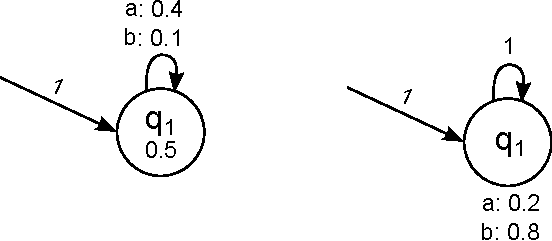
\includegraphics[scale=1]{./pictures/model-with-and-without-stop-symbols.pdf}
\caption{A \gls{pa} and \gls{hmm}.}
\label{fig:model-with-and-without-stop-symbols}
\end{centering}
\end{figure}

We will now consider the probability distributions both models define to observe the difference implied by the halting probability of the \glspl{pa}.
With the \gls{pa}, we can calculate the probability of generating an empty sequence, simply by starting in state 1 and stopping immediately before emitting any symbols. That is, $P_{PA}(\varepsilon) = 0.5$. We can also produce non empty sequences. For instance, we have that $P_{PA}(a) = \pi_1\phi_{1,a,1}F_1 = 0.2$, where $\pi_q$ is the probability of starting in state $q$, $F_q$ is the probability of stopping right after entering state $q$, $\phi_{q,s,q'}$ is the probability of going from state $q$ to state $q'$ while emitting the symbol $s$.
In the same manner, we get that $P_{PA}(b) = 0.05$.
If we in this way calculate a probability for all possible sequences, we will see that all of those probabilities sum up to 1. Thus, the \gls{pa} defines a probability distribution over $\Sigma^\ast$\cite{Dupont:2005:LPA:1746577.1746601}.

When we turn our look to the \gls{hmm}, we see that its structure looks very much like the structure of a \gls{pa}.

Without stop probabilities, the probability definition it defines should not be interpreted in the same way as for the \gls{pa}. For instance, it does not make sense to define the probability of the empty sequence $P_{hmm}(\varepsilon)$. Also, if we start to calculate the probabilities of particular sequences in the straight forward way, we get that $P_{HMM}(a) = 0.2$, $P_{HMM}(b) = 0.8$. It is easy to see, that the missing stop probabilities causes the following property to hold:

\[\forall n, \sum_{w \in \Sigma^n} P(w) = 1\]

This means, that in contrast to the \gls{pa}, the \gls{hmm} defines a probability distribution over $\Sigma^n, \forall n \in \mathbb{N}$~\cite{Dupont:2005:LPA:1746577.1746601}.

The test data of the Pautomac competation should be assigned probabilities according to a distribution over $\Sigma^\star$.
This is both stated on the Pautomac website, but could also be determined from the fact that the test set contains empty sequences. However, some small modifications allow the \gls{hmm} to behave equivalent to the \gls{pa}, in terms of defining a probability distribution over $\Sigma^\ast$. One way is to add a new symbol $x$ to $\Sigma$, which should be interpreted as a stop symbol. The symbol $x$ is then added to the end of all sequences, including the empty sequence. Instead of using a stop symbol, one could also add a single final state with no emission probabilities and no out transitions~\cite{Dupont:2005:LPA:1746577.1746601}.